\documentclass[../thesis.tex]{subfiles}


\begin{document}

\chapter{The Prototype}\label{the_project}
The goal of this project is to create a prototype of a system that can generate voice commands
for talon from a source file in a given program language to the increase accuracy and efficiency of programming.
The result should take the form of a server that can be easily integrated into any editor as a plug-in
which handles the generation of voice commands and the communication with talon.
While the final version of the system should be general enough to handle any language, and be integratable with any the editor,
the prototype only aims to handle the \textit{Elm} programming language in the \textit{Neo-vim} editor.
This chapter will describe the design and architecture of the system.

\section{System Overview}%
\label{sec:voice_command_generation}
This section will provide an overview of the main functionalities of the system,
each of which will be discussed in more detail in their own sections.

\paragraph{Classified Identifier Extraction:}%
\label{par:classified_identifier_extraction}
The primary feature of the system is to expose information about the code being edited
to Talon such that the user can dictate high-level commands with a limited vocabulary
specific to the code being edited with high accuracy.
Perhaps the most important feature is the ability to keep updated talon lists
of identifiers in different classes. For example, you might have a list \textit{user.functions} which would contain
all the functions that are in scope in the file being edited.
Then you could define a voice command such as 
\begin{verbatim}
function {user.functions}: insert(functions)
\end{verbatim} 
which would provide the user with a way to insert a known function from a limited vocabulary which would increase the accuracy.
Given the code in \Vref{listing:elm_simple}, the list \textit{user.functions} might contain ``update'' and ``view''
(which were defined in this file), as well as ``onClick'', ``button'', ``text'' and ``div'' (from the import statements).
As we saw in the section on~\nameref{sec:elm}, there are other ways functions can be introduced
besides explicit declaration and imports, so some extra work is required define all relevant functions.
% Additionally, not all function names are pronounceable, so this must also be handled as discussed in Section~\ref{spoken_identifier_algorithm}.
% TODO

\paragraph{Code Navigation:}%
\label{code_navigation}
An integral part of editing code is moving the cursor between different parts of the program.
Having made Talon aware of the contents of the program being edited, we can enable
high-level voice commands for code navigation.
For example, navigating using the search functionality of the editor can be improved
by having a voice command that uses the list of known identifiers.
\begin{code}{text}{Simple Search Command}{symbol_search}
search <user.identifier>: 
    edit.find()
    insert(identifier)
    key(enter)
\end{code}
This can be improved even further by making the system aware of the
location and class of these identifiers.
A command like ``go function hello'' could move the user directly to the definition of the function named \textit{hello}.
This is much more efficient than using the search functionality because the user would not have to
consider whether or not there are occurrences of the same word between the current cursor position
and the target location.
% How to enable high-level code navigation commands?

\paragraph{Structural Editing:}%
\label{structural_editing}
While it is easy to make voice commands for making simple edits such as deleting whole lines,
programming often involves editing chunks of text that start in the middle of a line
and spans multiple lines. 
For mouse users it is quite simple to simply mark the start and end of any section, but for 
users of keyboard or voice commands this might require many more steps.
Since the target of these edits often corresponds to a node in the AST, this process
can be made much more efficient by enabling the users to utilize high-level editing commands
such as ``delete next case expression'', or ``delete type signature''.
This has potential for making certain editing activities much more efficient and intuitive,
as well as providing a more pleasant and natural user experience.

\section{Classified Identifier Extraction}%
\label{sec:classified_identifier_extraction}
This section should cover in detail what identifies should be extracted
and how this is accomplished. \Vref{tab:constructs_of_interest} shows
what identifiers should be tracked, and which constructs they can be found in.
For example, a function can be declared directly, imported from another module, are generated
from type declarations. The notation \textit{Type [Alias] Declaration} is a shorthand
for writing both \textit{Type Declaration} and \textit{Type Alias Declaration}.
Tracking these classes of identifiers should be sufficient for Elm, but more
might be added to how do more programming languages in the future.
The following section will explain in detail how each of these classes of identifiers
are extracted, and how they might be used in voice commands.
% As all of the identifer classes may be found in import statements, imports will be covered
% separately in Section~\ref{imports}.

\begin{table}[htpb]
    % \centering
    \begin{tabular}{|c|c|}
        \hline
        Construct & Found In \\
        \hline
        % add a column for reference
        Function & Function Declaration, Import, Type [Alias] Declaration \\
        Variable & Function Declaration, Import, Type [Alias] Declaration \\
        Constructor & Type [Alias] Declaration \\
        Type & Type [Alias] Declaration, Import \\
        Module & Dependency, Import, Implicit Import \\
        Record Field & Record Type, Record Literal \\
        \hline
    \end{tabular}
    \caption{Constructs of Interest}
    \label{tab:constructs_of_interest}
\end{table}

\subsection{Identifer Classes}%
\label{sub:identifer_classes}
This section will provide a more in-depth explanation of the different identifer classes from Table~\ref{tab:constructs_of_interest}. 

\subsubsection{Functions, Variables and Constructors}%
\label{par:functions_and_variables}
Functions, variables and constructors are all normal ``values'' in Elm, but have some properties
that needs to be taken care of in this context.
There is no way to differentiate between functions and variables syntactically due to the higher order nature of the language.
The only way to tell if a value is a function is to protect its type, which is not always available easily.
It is debatable whether or not it is necessary to separate these two classes for the particular use case we have in mind,
but we mention it as a possible capability of the system.
The advantage is that we can further limit the vocabulary in commands such as:
\begin{verbatim}
call <user.function>: user.call_function(function)
\end{verbatim}
More important however is the difference between constructors and other values.
In elm it is not possible to declare a function with an uppercase first letter.
This is to make it easier to distinguish constructors from regular functions.
It is however possible to have a function with the same name as a constructor, only with different formatting.
Because we would like to have a way of distinguishing between declarations like the one seen in \Vref{box_example},
we need to track constructors separately.
\begin{code}{elm}{}{box_example}
type Box = Box Int

box i = Box (i + 1) 
\end{code}

\subsubsection{Types}%
\label{par:types}
As in most ML-style languages, types play an central role in Elm programming.
Since Elm has global type inference, and the type system is simple enough that
well-typed expressions are usually unambiguous, type signatures can be generated
automatically which seemingly would make the ability to dictate signatures unnecessary.
Automatically generating tab signatures is possible in IntelliJ, but the Elm LSP does not have this feature. 
It will probably be implemented in the future.
Regardless, programmers would often want to type out the signatures manually for a few reasons.
Adding the type signature before writing the function body helps the compiler provide better
error messages along the way when writing complex definitions.
Additionally, the generated signature might not use all the type aliases the programmer intended, and
type variables would have to be renamed.
By tracking the known types, dictating type signatures can be made extremely efficient.

\subsubsection{Modules}%
\label{par:modules}
The two main use cases for keeping a list of modules is to dictate imports, and referencing functions in those modules.
The full list of modules available to the user can be found by retrieving the packages using the project, as described in Section~\ref{sub:dependencies}.
% check if core is listed here
% also user-defined modules
Given a module \textit{Array} with a function called \textit{append}, the user should be able to
reference this function with the phrase ``array append'', which would produce the output \textbf{Array.append}.
Explicitly dictating the \textbf{.} can optionally be done to disambiguate in certain scenarios, but should usually not be necessary.

Voice commands should also be aware of import aliases.
If the Array module instead was imported as
\begin{minted}{elm}
import Array as A
\end{minted}
the phrase ``array append'' should instead produce the output \textbf{A.append}.
It should also be possible to reference the function using the alias (i.e ``A append'').

\subsubsection{Record Fields}
Record fields should be tracked for the same reason we track functions.
Given the following decorations:
\begin{minted}{elm}
type alias Person = { name : String }

john : Person
john = ...
\end{minted}
it should be possible to enter \textit{john.name} by saying ``John dot name''.
Elm also has syntax for record access functions, so the phrase ``dot name'' can be used to
refer to the function \textit{.name}.
Since Elm support anonymous records, to find all possible record fields we also need to check
any record literal and destructuring declaration.
Note that the type of the value \textit{john} is not necessarily relevant unless we
aim to make the voice commands aware of the types as well.% referred to discussion on this in general
This can be achieved with the following voice commands:
\begin{verbatim}
<user.value> [dot] <user.record_field>: "{value}.{record_field}"
dot <user.record_field>: ".{record_field}"
\end{verbatim}

\subsection{Extracting with Regular Expressions}
Regular Expressions are perhaps the simplest and most well-known tool for capturing parts of text according to given rules.
The following regular expression captures the name of types from the regular type declarations and type alias declarations:
\begin{verbatim}
type (?:alias )?(?<type>[A-Za-z]+)
\end{verbatim}
This expression creates a capture group named ``type'' which matches sequences of lower and upper case letters
that are preceded by the keyword \textit{type} and optionally the keyword \textit{alias}.
It is worth considering regular expressions as a solution to the identifier extraction problem
considering the ubiquitous nature of regular expression engines and libraries, but they do have some serious limitations.
Regular expressions recognize regular languages, but the main subject of analysis is programming languages
which usually have a context free syntax.
While this does not necessarily mean that they will be insufficient for any particular analysis
it does mean they can't recognize recursive patterns which are prevalent in the syntax of programming languages.
Seemingly simple rules such as that a pattern should not occur within the string literal are often
hard to express and requires advanced features like lookahead/lookbehind.
Attempting to achieve higher granularity often results in complex and difficult to read expressions
which make them impractical for certain use cases.

Therefore, regular expressions are probably not well-suited for identifier extraction for Elm, but might be for simpler languages
such as LaTex or Markdown, or for early iterations/prototypes of implementations for any given language.


\subsection{Extracting From Documentation}%
\label{sub:dependencies}
The vast majority of code used in a project will not be written by the project author, but will be available
through a package. It is very important that the system is aware of packages the user is depending on, what modules can be found in these packages, 
and which identifiers are exposed by these modules. Extracting information from the documentation is generally a simpler problem
than extracting from source files because the data is exposed in a simpler format (json) which is much easier to parse then Elm source code.
This section explains how we can analyze the Elm documentation to provide useful voice commands.

The \textit{dependencies} field of the \textit{elm.json} file lists all the packages the authors of this project
are using directly.
There is a separate field for indirect dependencies, also known as transitive dependencies, 
but we are only interested in the direct dependencies because those are the ones the user might want to
reference in their programs.
The documentation to all packages in Elm is readily available by making a request to
\textit{https://package.elm-lang.org/packages/<author>/<name>/<version>/docs.json}.
Each documentation file is a list of module objects.
The contents of these module objects along with an explanation can be seen in table~\ref{tab:documentation_fields}.

\begin{table}[htpb]
    \centering
    \begin{tabular}{|c|c|}
        \hline
        Field & Explanation \\
        \hline
        name & The name of the module \\
        comment & Documentation text for the module \\
        unions & Type Declarations \\
        aliases & Type Alias Declarations \\
        values & Value Declarations (functions/constants) \\
        binops & User-defined binary operators \\
        \hline
    \end{tabular}
    \caption{Module Structure in docs.json}
    \label{tab:documentation_fields}
\end{table}

% \subsubsection{Snippets}% figure out how to use coc lists

\Vref{array_excerpt} shows parts of the first module entry from \textit{elm/core}.
\begin{code}{json}{Excerpt from docs.json}{array_excerpt}
  {
    "name": "Array",
    "comment": " Fast immutable arrays. (...)",
    "unions": [
      {
        "name": "Array",
        "comment": "Representation of fast immutable arrays.",
        "args": ["a"],
        "cases": []
      }
    ],
    "aliases": [],
    "values": [
      {
        "name": "append",
        "comment": "Append two arrays to a new one. (...)",
        "type": 
            "Array.Array a -> Array.Array a -> Array.Array a"
      },
      ...
    ],
    "binops": []
  }
\end{code}
The rest of this sections will explain each of these fields in more detail.
All of the following examples will be from \textit{elm/core}.

\subsubsection{Unions}\label{unions}
The \textit{unions} field contains the exposed type declarations and their constructors.
The word \textit{unions} refers to the fact that elm types are \textit{disjoint union types}, or \textit{tagged unions}.
A type declaration like in the one in \Vref{maybe} would produce the union field in \Vref{maybe_json}.
% \begin{minted}{elm}
% type Maybe a
%     = Just a
%     | Nothing
% \end{minted}
% would produce a union field like this: 
\begin{code}{ json }{Maybe JSON}{maybe_json}
{
  "name": "Maybe",
  "comment": " Represent values that may or may not exist. (...)",
  "args": ["a"],
  "cases": [
    ["Just", ["a"]],
    ["Nothing", []]
  ]
}
\end{code}
The \textit{args} field is a list of the names of the type parameters.
A nonempty args indicates a polymorphic data type.
There might be something to do with the name of these type arguments, but for now they will be ignored.
The \textit{cases} field is a list of constructors for the type.
Each entry is a pair of the name of the constructor and list of the types of the arguments to that constructor.
Constructors with no arguments are constants, otherwise they are functions.

\subsubsection{Aliases}\label{aliases}
\textit{Aliases} is a list of type alias declarations.
This entry is very simple.
There is a \textit{type} field, which indicates which type is being aliased, and the name.
We are only interested in the name field.
A type alias like
\begin{minted}{elm}
type alias Id = Platform.ProcessId
\end{minted}
would produce the alias field in \Vref{processid}.
\begin{code}{json}{Platform.ProcessId JSON}{processid}
{
  "name": "Id",
  "comment": " A light-weight process that runs concurrently. (...)",
  "args": [],
  "type": "Platform.ProcessId"
}
\end{code}

\subsubsection{Values}\label{values}
The \textit{values} field contains all the functions and constants in the module.
One such example can be seen in \Vref{head_funk}.
\begin{code}{json}{Value Declaration JSON}{head_funk}
{
  "name": "head",
  "comment": " Extract the first element of a list. (...)",
  "type": "List.List a -> Maybe.Maybe a"
}
\end{code}
Since functions are normal values, we need to look at the type to distinguish functions from constants.
We can see that \textit{head} is a function from the use of the function type constructor (->).
It is however not as simple as checking whether (->) occurs in the type.
The type
\begin{minted}{elm}
List (a -> a)
\end{minted}
denotes a list of functions, but is not a function itself.
Determining what values are functions therefore requires more sophisticated parsing of the type signature.
% reference: where do I explain this?

\subsubsection{Binary Operators}\label{binary_operators}
The \textit{binops} field contains the binary operators in that module.
These entries are similar to \textit{values}, but also contain \textit{precedence} and \textit{associativity}.
\begin{code}{json}{Cons Operator JSON}{cons}
{
  "name": "::",
  "comment": " Add an element to the front of a list. (...)",
  "type": "a -> List.List a -> List.List a",
  "associativity": "right",
  "precedence": 5
}
\end{code}
In some languages, such as PureScript, infix operators are defined as aliases
for regular functions which ensures that each operator has a canonical way of referencing it vocally.
Since elm does not have this property, this connection is to be made another way.
The operator in this example is historically referred to as \textit{cons}, but it could also be called
\textit{prepend} if you want the name to be more descriptive.
Elm support declaring infix operators, but normal users can not define operators as of version 0.19, so this might not be a problem in practice.
Most operators are defined in \textit{elm/core}, but not all.% |., |=
A reasonable way to this might be to checked operators found in packages against the talon list
and warn the user if an operator is found, but has no way to be dictated.

\subsection{Extracting From Language Server}%
The Language Server Protocol defines two methods for requesting information about the symbols in the project: \textit{Document Symbols} and \textit{Workspace Symbols}.

\paragraph{Document Symbols} retrieves information about symbols in the file currently being edited.
The responses is a list of objects describing symbols with information about where it is in the file
and what kind of symbol it is. \Vref{document_symbols_entry} shows the entry for the main function in an Elm program.
\begin{code}{ json }{Document Symbol Entry}{document_symbols_entry}
{
  "lnum": 16,
  "col": 1,
  "range": {
    "end": { "character": 9, "line": 21 },
    "start": { "character": 0, "line": 15 }
  },
  "level": 0,
  "kind": "Function",
  "containerName": null,
  "text": "main"
} 
\end{code}

\paragraph{Workspace Symbols} retrieves information about symbols and entire project.
This also includes symbols in packages the project depends on.
Because of this, LSB might eliminate the need to analyze documentation directly for some use cases.
This is however not always the case as the workspace entries provides less information than the documentation.
The entries are similar to those of the document symbols, but because there will be a lot more entries some
information is left out (such as line number), and the kind uses an ID instead of the name.
The location field also has a \textit{uri} which tells which file the symbols from.
This can be used to determine the package and module the symbol is from.
\begin{code}{json}{Workspace Symbols Entry}{workspace_symbols_entry}
{ 
  "location": {
  "uri":
    "file:///<HOME>/.elm/0.19.1/packages/elm/json/1.1.3/src/Json/Encode.elm",
  "range": {
    "end": { "character": 93, "line": 169 },
    "start": { "character": 0, "line": 167 }
    }
  },
  "name": "array",
  "kind": 12 
}
\end{code} 

\subsubsection{Integration}% this section needs more work
Integrating with the language server is very simple, especially if the editor in question allows users to easily
call functions from the plug-in that acts as the LSP client.
\Vref{vim_lsp} shows how you can define a function that requests the workspace symbols from the server and saves the result
to a file.
\begin{code}{vim}{Simple Vim LSP integration}{vim_lsp}
function SaveWorkspaceSymbols()
    let symbols = CocAction('getWorkspaceSymbols')
    let symbols = json_encode(symbols)
    let file = "/Users/gauteab/uio/master/thesis/workspaceSymbols.json"
    call writefile([symbols], file)
endfunction
\end{code}
This can easily be extended to a full integration with the system.

\subsubsection{Limitations}
While using the LSP for extracting identifiers is convenient, it will likely be insufficient in terms of feature completeness in some cases.

LSP does not expose information about the file that does not pertain to a symbol.
It would therefore not be as useful for implementing navigation and structural editing.

Additionally, the implementations for different languages vary greatly in how feature-rich they are, and not all language servers support document symbols and workspace symbols.
Many servers are in active development so this is likely to change at some point.



\subsection{Extracting With TreeSitter}
Being a general purpose parsing system, TreeSitter easily enables arbitrary syntactic analysis.
Once the parser for the given programming language has been acquired, getting the parse tree
is very simple.
Then one could simply traverse the tree and extract identifiers from the nodes directly.
This approach is straightforward, but manually defining the traversal take some extra work.
Using the Query API of TreeSitter, this can be greatly simplified.
% This section shows how TreeSitter Queries can be used to extract identifiers from a Elm source file.

\subsubsection{Using TreeSitter with Elm}
The parser for Elm is available at \url{https://github.com/elm-tooling/tree-sitter-elm}
and is also available as a npm package at \url{https://www.npmjs.com/package/tree-sitter-elm} for simple installation
for projects using the \textit{Node.js} bindings.
A simple Elm declaration like
\begin{minted}{elm}
greet name = 
    "Hello " ++ name
\end{minted}
would be represented by the following TreeSitter S-expression:
\begin{verbatim}
(value_declaration functionDeclarationLeft: 
 (function_declaration_left (lower_case_identifier) 
  pattern: (lower_pattern (lower_case_identifier))) (eq) 
    body: (bin_op_expr part: (string_constant_expr (open_quote) 
     (regular_string_part) (close_quote)) part: 
     (operator (operator_identifier)) part: 
       (value_expr name: (value_qid (lower_case_identifier)))))
\end{verbatim}
Note that it is a quirk of this implementation that all terminals in the grammar are named.
Therefore nodes like \textit{(eq)} and \textit{(open\_quote)} are included in
the textual representation of the tree, and you cannot use the \textit{is\_named} function
to identify terminals when traversing the tree in code.
This is unlikely to be a problem, but if it is it can be resolved by a simple change in the grammar.

The rest of this section will show how identifiers can be extracted from an Elm source file using TreeSitter Queries.

\subsubsection{Types}
The following query finds the name of all types available in the given file:
\begin{verbatim}
(exposed_type (upper_case_identifier) @type)
(type_declaration (upper_case_identifier) @type)
(type_alias_declaration (upper_case_identifier) @type)
\end{verbatim}
The query consists of three parts.
Each of them matches an \textit{upper\_case\_identifier} and assigns to it the label \textit{type}.
The first one finds types in import statements, and the second and third finds names from regular type declarations
and type alias declarations respectively.

\subsubsection{Constructors}
Constructors can be extracted from type declarations with a simple query:
\begin{verbatim}
(union_variant) @constroctor
\end{verbatim}
This would extract the whole constructor including parameter types, which could be used to distinguish
between callable constructors and constants.
If one were only interested in the name of the contractor that could be extracted with the following query:
\begin{verbatim}
(union_variant (upper_case_identifier) @constroctor)
\end{verbatim}

\subsubsection{Values}
As TreeSitter only enable syntactic analysis we cannot distinguish between functions and other values
without implementing the Elm type system as part of that analysis.
Due to the variable naming rules of elm, the values in the program can be extracted with a very simple query:
\begin{verbatim}
(lower_case_identifier) @value
\end{verbatim}
This is a very simple solution, but there might be need for a more granular query.
For example, this query would match the last part of a qualified identifier like
\begin{minted}{elm}
Browser.sandbox
\end{minted}
as well as type variables.
A more granular query can be made to only include the desired kinds of lowercase identifiers:
\begin{verbatim}
(function_declaration_left (lower_case_identifier) @value)
(exposed_value) @value
(lower_pattern) @value
\end{verbatim}
\textit{function\_declaration\_left} refers to the left-hand side of an assignment, so the first part of the query refers to the name of functions.
The second part finds values in import statements, similarly as the first part of the type of query.
The last part \textit{(lower\_pattern)} refers to variable names in pattern matching expressions as well as the parameters of function declarations.
In the following declaration:
\begin{minted}{elm}
unwrap : Maybe value -> value
unwrap maybeValue =
    case maybeValue of
        Just content ->
            content
        Nothing ->
            Debug.todo "trying to unwrap nothing"
\end{minted}
the query would find \textit{unwrap}, \textit{maybeValue} and \textit{content}, but not \textit{value} or \textit{todo}.

\subsubsection{Modules}
Extracting module names can be done with a simple query like:
\begin{verbatim}
(import_clause 
    (upper_case_qid (upper_case_identifier) @module))
(import_clause 
    (as_clause (upper_case_identifier) @module-alias))
\end{verbatim}
This would find all identifiers used in module names in the import statements as well as the module aliases from \textit{as clauses}.
If one wanted to merge these two classes that could be achieved simply by renaming the \textit{module-alias} capture to \textit{module}.

More advanced use cases needs to keep the connection between module aliases and the module from which it was created.
For the system in question this is indeed the case because we want to use the alias as part of the command for dictating functions in that module.
To achieve this one could simply extract the whole node containing the alias, and extract the relevant parts in code.
A query like:
\begin{verbatim}
(import_clause (as_clause)) @import-with-alias
\end{verbatim}
will capture any import statement with an alias.
Once this node has been retrieved you can access the relevant parts of the tree directly:
\begin{minted}{js}
module = node.children[1]
alias = node.children[2].children[1]
\end{minted}

\subsubsection{Record Fields}
Extracting record fields from record types is very simple:
\begin{verbatim}
(field_type (lower_case_identifier) @record-field)
\end{verbatim}
Since elm has anonymous record types, there might be situations where record fields are used
without having been declared or imported.
For example in the declaration
\begin{minted}{elm}
f {a, b} = a.c.d
\end{minted}
we can see from the record destructuring expression \textit{\{a, b\}} that \textit{a} and \textit{b} are both used as record fields,
and from the field access expression \textit{a.c} we can see that \textit{c} and \textit{d} are also record fields.
These two cases can be captured by the following query:
\begin{verbatim}
(record_pattern (_ (lower_case_identifier) @record-field))
(field_access_expr (lower_case_identifier) @record-field)
\end{verbatim}



% \subsubsection{Imports}\label{imports}
% Example~\ref{ex:import} shows an complex import statement which imports the \textit{Html.Events} module,
% introduces an alias (\textit{Events}) and also import one of the members of the module (\textit{onClick}).
% After processing this statement, \textit{Events} would be added to the list of active modules, 
% and \textit{onClick} would be added to the list of active functions.
% \begin{example}[Complex Import]\label{ex:import}
% \begin{minted}{elm}
% import Html.Events as Events exposing (onClick)
% \end{minted}
% \end{example}

% \subsection{Spoken Identifier Algorithm}\label{spoken_identifier_algorithm}
% Describe convert a formatted identifier into a form recognizable by talon.

\section{Voice Command Optimization}
Simply extracting identifiers should result in a significant improvement, but there are still some cases
where the naïve commands generated as described above could be improved upon.
This section will discuss a few methods for achieving higher accuracy and shorter voice commands.

\subsection{Automatic Acronyms}\label{automatic_acronyms}
If an identifier is very long, its name might not be the most efficient way to refer to it.
An identifier like \textit{processAnalysisResults} consists of three words, but is eight syllables long.
A common way to enter long identifiers is to rely on the auto complete feature of the editor.
Entering ``p a r'' is usually sufficient to have the correct identifier as one of the top results for the auto-complete.
Then the user would have to say the command used for triggering the auto-complete.
This is a useful workaround for long identifiers with hard to pronounce words, but it takes extra time
due to the user having to wait for the auto-complete to activate.
This pattern of use can be subsumed by this system by generating acronyms for long identifiers.
By splitting identifiers by words, taking the first letter of each word, and adding this as an extra key
for that identifier, users should be able to dictate more complex identifiers in shorter amounts of time.
% maybe discuss the structure of identifiers (with respect to how to split them)

\subsection{Prefix Elimination}\label{prefix_elimination}
A common idiom in some programming languages is to have the start of an function name refer to the ``thing''
or datatype on which it operates. This is mostly common in languages without user-defined name spaces such as \textit{C}
, but is also common in higher-level languages when a few functions share a domain, but they do not warrant
being move to their own module/package.
For example, if you have two functions \textit{handleHttpConnection} and \textit{handleTcpConnection}, and no other
functions/variables containing the name \textit{HttpConnection} or \textit{TcpConnection}, you might want to
be able to refer to those functions using only the suffix (without the ``handle'' prefix).
This would be a relatively minor optimization, but nevertheless worth considering.

\subsection{Overrides}\label{overrides}
Not all identifiers will be perfectly pronounceable.
Programmers often use domain specific vocabularies filled with words not used in normal English.
For example the word \textit{json} is actually an acronym for ``JavaScript Object Notation'', but is rarely
pronounced ``J S O N''.
People will pronounce it as either ``J son'' (or ``jay son''), or as the name ``Jason''.
Talon can recognize the first version most of the time, but it might require more precise enunciation from the user.
The name Jason is easily recognizable, so overriding the word json with Jason will give higher overall accuracy.
A simple solution to this problem is to allow users to declare a list of overrides for which the system
can do a simple lookup to make substitutions in the final stage of command generation like so:
\begin{minted}{json}
{
  "overrides": {
    "json": "Jason",
    "init": "in it"
  }
}
\end{minted}
The list of overrides can be partially filled automatically by extracting the list of abbreviations and homophones
from the users Talon configuration files.


% TODO: Find example of words talon can't recognize

% \subsection{Local Bindings}%
% \label{sub:local_bindings}
% Should local bindings be handled differently from top level bindings?

\section{Code Navigation}%
\label{sec:code_navigation}
Once information has been extracted from the program, enabling high-level navigation commands is quite simple.
\Vref{symbol_navigation} shows how you could create talon commands that uses the classified identifiers
to implement a simple grammar that allows for navigation that takes the type of the navigation target
into account.
\begin{code}{text}{Navigational Commands for Symbols}{symbol_navigation}
go to { user.symbol_identifier }:
    user.symbol_navigate("{symbol_identifier}", "identifier")
go type {user.symbol_type}:
    user.symbol_navigate("{symbol_type}", "type")
go fun {user.symbol_function}:
    user.symbol_navigate("{symbol_function}", "function")
\end{code}
The action \textit{symbol\_navigate} queries the server
for the position of the identifier with name matching the first parameter, and type matching the second.
It will then trigger \textit{editor\_go\_to\_position} which in the context of the current editor
to the beginning of that symbol.

Since we have access to the entire parse tree, it is also possible to navigate two nodes that
are not associated with any given identifier.
This would not be possible with an implementation that only uses LSP.
\begin{code}{text}{Navigational Commands for Non-symbols}{literal_navigation}
go import: user.symbol_navigate("", "import")
go string: user.symbol_navigate("", "string")
go number: user.symbol_navigate("", "number")
\end{code}

\paragraph{Context aware navigation}
can be achieved simply by exposing the cursor position to Talon.
When a query is executed, the response from the server will be the node
which is closest to the cursor. By also keeping track of
the previous query and its results, you can also have
the commands that cycle through results in order to quickly navigate
when the query can capture multiple nodes.
\begin{verbatim}
go to next: user.go_to_next_result("forward")
go to last: user.go_to_next_result("backward")
\end{verbatim}
% Given the following program snippet:
% \begin{minted}{elm}
% type Update
%     = SoftwareUpdate
%     | FirmwareUpdate

% update : Msg -> Model -> Model
% update msg model = ...
% \end{minted}


\section{Structural Editing}%
\label{sec:structural_editing}
Structural editing can easily be achieved by building upon the implementation of navigation.
By implementing an action to select a given range in the editor, you can create commands
that select nodes based on their type and associated identifiers in the same manner as with navigation.
For example, to delete the typed declaration in Vim, you can create a command that captures the name of the type declaration,
selects it, and presses ``d'' in order to delete it.
\begin{verbatim}
delete type {user.symbol_type}: 
    user.symbol_select("{symbol_type}", "type")
    key(d)
\end{verbatim}
Structural editing capabilities can be implemented either client-side, server-side, or in Talon.
There are certainly trade-offs to each approach, but I will not go into detail on this issue.
For the prototype the editing commands were implemented in Talon.


% \section{Design Goals}%
% \label{sec:design_goals}
% configurable, accuracy, intuitive/consistent (user should not have to look up the generated commands), 
% shortest commands possible

\section{Architecture}%
\label{sec:architecture}
The system consists in total of three parts: Talon scripts, The Server and a Vim extension (Client).
The server is responsible for parsing source files and extracting information using TreeSitter,
as well as performing normalization on the extracted identifiers in order to make them
more recognizable before sending them to Talon.
The Vim extension manages the window title which is used by Talon to track information about the
current editor state such as current mode and cursor position. Additionally, it will notify
the server whenever an Elm document is either opened, closed or written to.
The talon scripts defines voice commands that utilizes the information received from the server
and defines actions to query the server for information about a given identifier.
An overview of the system can be seen in Figure~\ref{fig:architecture}.

\begin{figure}[htpb]
    \centering
    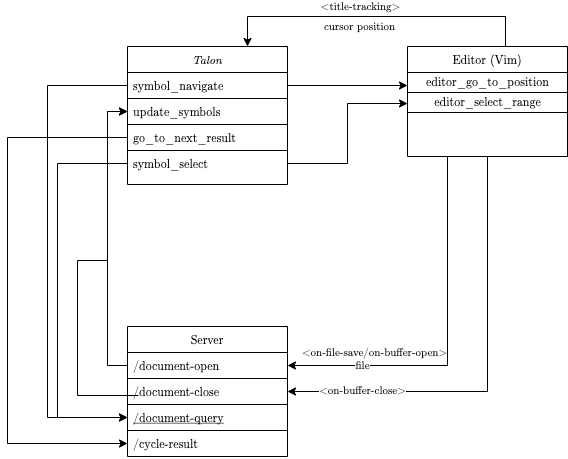
\includegraphics[width=0.8\linewidth]{images/architecture.png}
    \caption{System Architecture}%
    \label{fig:architecture}
\end{figure}

\section{Implementation Details}%
\label{sec:implementation}
This section presents information about the prototype in it's current state as well as reasoning behing the tools and techniques used.
% implementation details such as programming language etc
\subsection{Tools}%
\label{sub:tools}
For the purpose of this prototype I chose to use TreeSitter because it provides full information about the program
being analyzed, whereas LSP only exposes information about symbols which does not enable the use of
syntactic elements such as literals and if expressions as navigation targets.

\subsection{Programming Languages and Frameworks}
The main consideration with regards to choice of programming language for the server of this project is the availability of high-level bindings to the TreeSitter library.
Using the C library directly would also have been a possibility, but going with a higher level language will likely result in a more reliable result.
Of the handful of languages that has this, the \textit{Node.js} seems to be one of the most stable and mature.
In order to get static type safety, PureScript was chosen over the dynamically typed JavaScript.
TypeScript could also have been used to accomplish this, but PureScript has a stronger type system.
Additionally, PureScript being a pure functional language similar to Haskell provides even stronger runtime guarantees.
\textit{HTTPure}, a HTTP framework for PureScript, was used to develop the server.

\subsection{Platforms}
The prototype is multiplatform and has been tested on MacOS (Catalina and BigSur), Linux (Ubuntu) and Windows 10.

\subsection{Interprocess Communication}
Talon does not currently have any officially recommended way of handling communication with external programs.
There has been discussion of implementing some kind of RPC in Talon.
Currently there are two ways the server can send commands to Talon.
By using the \textit{Node.ChildProcess} API, the server can spawn an instance of the Talon REPL (\textit{~/.talon/.venv/bin/repl}).
This server can then simply pipe an action into the REPL as a string.
The other method is to write the action to be executed to a file that is being watched by Talon using the \textit{fs.watch}
method. Whenever the file is written to, Talon will pick up on the change and execute action within that file.
The latter is slower, but was used in the Windows implementation due to permissions issue executing the Talon REPL from within Windows Subsystem Linux (WSL).



\subsection{Project Statistics}%
\label{sub:project_statistics}
This section briefly present some data about the implementation of the prototype.
Table~\ref{tab:stats} shows the amount of code written per programming language.
This is worth noting because it shows how much of the system is implemented in the different parts
(Editor, Server and Talon).
The same information is presented in Figure~\ref{fig:lang_dist}.
Not included in these figures are the talon files that defines the grammar for the voice commands,
and talon extensions written by other users that were slightly modified and extended such as the Vim integration from \url{https://github.com/fidgetingbits/knausj_talon
}.

% \begin{figure}[!ht]
%   \label{distribution}
%   \centering
%   % \rule{6.4cm}{3.6cm}
%   % \qquad
%   \begin{tabular}{|c|c|c|}
%       \hline
%       Language&Files&Lines\\
%       \hline
%       PureScript&8&626\\
%       Python&3&210\\
%       JavaScript&6&32\\
%       VimScript&1&31\\
%       \hline
%       Total&18&899\\
%       \hline
%   \end{tabular}
%   \subfile{chart}
%   % \captionlistentry[table]{A table beside a figure}
%   \captionsetup{labelformat=andtable}
%   \caption{Language Distribution}
% \end{figure}

\begin{table}[htpb]
    \centering
    \begin{tabular}{|c|c|c|}
        \hline
        Language&Files&Lines\\
        \hline
        PureScript&8&626\\
        Python&3&210\\
        JavaScript&6&32\\
        VimScript&1&31\\
        \hline
        Total&18&899\\
        \hline
    \end{tabular}
    \caption{Files and lines per language}
    \label{tab:stats}
\end{table}


\begin{figure}[htpb]
    \centering
    \subfile{chart}
    \caption{Language Distribution}%
    \label{fig:lang_dist}
\end{figure}

This shows that the server is by far the biggest part of the project (PureScript + JavaScript),
although a notable portion of this is the definition of the foreign function interface to TreeSitter (188 lines).
Most notably however it shows that the editor plug-in for Vim was a very small part of the work
which should serve as an indicator that implementing these features in other editors
it will be quite simple.
It also shows that the total amount of code needed to implement the features available in the prototype
is quite low, which speaks volumes about the ease-of-use of both Talon and TreeSitter.


% ===============================================================================
%  Language            Files        Lines         Code     Comments       Blanks
% ===============================================================================
%  JavaScript             &6          &32          &26           &0           &6
%  PureScript              8          626          442           82          102
%  Python                  3          210          142           26           42
%  VimScript               1           31           -             -            -
% ===============================================================================
%  Total                  18          899          610          108          150
% ===============================================================================
\section{Prototype Completeness}%
\label{sec:prototype_completeness}
This section outlines the future completeness of the final prototype with respect to
the features discussed previously in this chapter.
The source code for the prototype is publicly available at \url{https://github.com/Gauteab/talon-tree-sitter-service}.

\paragraph{Identifier Extraction:}
The current implementation only uses TreeSitter and is only able to work with a single file.
If the user opens a different file, the identifiers will be overwritten.
Ideally, the system would have one namespace further identifiers in the current file
and one for the whole project.
This is likely the biggest limitation of the current implementation.

Currently the system creates Talon lists for functions and type declarations as well as one for all identifiers using the query in \Vref{identifier_extraction_query}.
\begin{code}{text}{Final Identifier Extraction Query}{identifier_extraction_query}
(lower_case_identifier) @identifier 
(upper_case_identifier) @identifier
(function_declaration_left (lower_case_identifier) @function)
(exposed_value) @function
(lower_pattern) @function
(exposed_type (upper_case_identifier) @type)
(type_declaration (upper_case_identifier) @type)
(type_alias_declaration (upper_case_identifier) @type)
\end{code}
More queries have been written, but due to an issue with the Windows bindings for TreeSitter
that causes segmentation faults when the query string is too long, some of the queries
were not included in the prototype.
This can be fixed by splitting up the query string and running it as multiple queries.

\paragraph{Structural Navigation:}
Besides only being able to navigate within a single file, navigation is working very well.
Users can navigate using the type of the target node to disambiguate in their commands.
It is both possible to navigate to nodes with and without associated identifiers.
The currently available navigation targets are:
\begin{itemize}
    \item identifier
    \item type declaration
    \item function/value declaration
    \item import statement
    \item string literal
    \item number literal
\end{itemize}


\paragraph{Structural Editing:}
The prototype only supports very basic structural editing;
it is possible to select and delete functions and type declarations.
The capabilities of the server however should be enough to implement
more complicated editing commands such as moving nodes.

\paragraph{Voice Command Optimization:}
This chapter outlined three optimizations that could be made to maximize accuracy
and minimize verbosity: \nameref{automatic_acronyms}, \nameref{prefix_elimination}, and \nameref{overrides}.
Overrides has been fully implemented, while the other two are not implemented at all.
These require more complicated analysis, but are realistically achievable given a bit more time.

\section{Extending the System}%
\label{sec:extending_the_system}
The most important motivation for using TreeSitter was the availability
of parsers for many different languages.
This section outlines the steps required to add support for more languages and editors.
Do note that some re-factoring of the current code base might be required
to facilitate these changes.

\subsection{Adding Languages}
The steps required to add support for a new programming language are as follows:
\begin{enumerate}
    \item Install TreeSitter Parser
    \item Write TreeSitter Queries
    \item Add Language Specific Voice Commands
\end{enumerate}
The first step is very simple.
For example, to add Python support simply use npm to install the parser from \url{https://www.npmjs.com/package/tree-sitter-python}.

Writing queries is also quite simple, but requires some knowledge of the internal structure
of the parse tree.
There were two sets of queries: one for extracting identifiers, and a separate one
used for navigational commands.
For the most part writing these queries as a matter of mapping the names
in from the parse tree to the name you want users to dictate.
This process can be quite iterative; you only need a few queries to start using the system.

Step three is technically optional, but is recommended to get the most efficient commands set for the new language.
The existing commands should work as long as the new queries uses the same names as the ones currently implemented.

\subsection{Adding Editors}%
\label{sec:adding_editors}
As stated earlier, the vim plug in is very small should be easy to reproduce in a different editor.
There are two steps to making the system work in a different editor:
\begin{enumerate}
    \item Notify the server on file save
    \item Implement the editor actions for that context
\end{enumerate}
Notifying the server is done by making a HTTP call to the \textit{document-open} address with the filename.
There are currently three editor actions:
\begin{itemize}
    \item editor\_go\_to\_position(row: int, column: int)
    \item editor\_select\_range(line1: int, column1: int, line2: int, column2: int)
    \item editor\_get\_cursor\_position()
\end{itemize}
These are used for implementing navigation, editing and context awareness respectively.
It is not necessary to implement all of them.







\end{document}

